\documentclass[1p]{elsarticle_modified}
%\bibliographystyle{elsarticle-num}

%\usepackage[colorlinks]{hyperref}
%\usepackage{abbrmath_seonhwa} %\Abb, \Ascr, \Acal ,\Abf, \Afrak
\usepackage{amsfonts}
\usepackage{amssymb}
\usepackage{amsmath}
\usepackage{amsthm}
\usepackage{scalefnt}
\usepackage{amsbsy}
\usepackage{kotex}
\usepackage{caption}
\usepackage{subfig}
\usepackage{color}
\usepackage{graphicx}
\usepackage{xcolor} %% white, black, red, green, blue, cyan, magenta, yellow
\usepackage{float}
\usepackage{setspace}
\usepackage{hyperref}

\usepackage{tikz}
\usetikzlibrary{arrows}

\usepackage{multirow}
\usepackage{array} % fixed length table
\usepackage{hhline}

%%%%%%%%%%%%%%%%%%%%%
\makeatletter
\renewcommand*\env@matrix[1][\arraystretch]{%
	\edef\arraystretch{#1}%
	\hskip -\arraycolsep
	\let\@ifnextchar\new@ifnextchar
	\array{*\c@MaxMatrixCols c}}
\makeatother %https://tex.stackexchange.com/questions/14071/how-can-i-increase-the-line-spacing-in-a-matrix
%%%%%%%%%%%%%%%

\usepackage[normalem]{ulem}

\newcommand{\msout}[1]{\ifmmode\text{\sout{\ensuremath{#1}}}\else\sout{#1}\fi}
%SOURCE: \msout is \stkout macro in https://tex.stackexchange.com/questions/20609/strikeout-in-math-mode

\newcommand{\cancel}[1]{
	\ifmmode
	{\color{red}\msout{#1}}
	\else
	{\color{red}\sout{#1}}
	\fi
}

\newcommand{\add}[1]{
	{\color{blue}\uwave{#1}}
}

\newcommand{\replace}[2]{
	\ifmmode
	{\color{red}\msout{#1}}{\color{blue}\uwave{#2}}
	\else
	{\color{red}\sout{#1}}{\color{blue}\uwave{#2}}
	\fi
}

\newcommand{\Sol}{\mathcal{S}} %segment
\newcommand{\D}{D} %diagram
\newcommand{\A}{\mathcal{A}} %arc


%%%%%%%%%%%%%%%%%%%%%%%%%%%%%5 test

\def\sl{\operatorname{\textup{SL}}(2,\Cbb)}
\def\psl{\operatorname{\textup{PSL}}(2,\Cbb)}
\def\quan{\mkern 1mu \triangleright \mkern 1mu}

\theoremstyle{definition}
\newtheorem{thm}{Theorem}[section]
\newtheorem{prop}[thm]{Proposition}
\newtheorem{lem}[thm]{Lemma}
\newtheorem{ques}[thm]{Question}
\newtheorem{cor}[thm]{Corollary}
\newtheorem{defn}[thm]{Definition}
\newtheorem{exam}[thm]{Example}
\newtheorem{rmk}[thm]{Remark}
\newtheorem{alg}[thm]{Algorithm}

\newcommand{\I}{\sqrt{-1}}
\begin{document}

%\begin{frontmatter}
%
%\title{Boundary parabolic representations of knots up to 8 crossings}
%
%%% Group authors per affiliation:
%\author{Yunhi Cho} 
%\address{Department of Mathematics, University of Seoul, Seoul, Korea}
%\ead{yhcho@uos.ac.kr}
%
%
%\author{Seonhwa Kim} %\fnref{s_kim}}
%\address{Center for Geometry and Physics, Institute for Basic Science, Pohang, 37673, Korea}
%\ead{ryeona17@ibs.re.kr}
%
%\author{Hyuk Kim}
%\address{Department of Mathematical Sciences, Seoul National University, Seoul 08826, Korea}
%\ead{hyukkim@snu.ac.kr}
%
%\author{Seokbeom Yoon}
%\address{Department of Mathematical Sciences, Seoul National University, Seoul, 08826,  Korea}
%\ead{sbyoon15@snu.ac.kr}
%
%\begin{abstract}
%We find all boundary parabolic representation of knots up to 8 crossings.
%
%\end{abstract}
%\begin{keyword}
%    \MSC[2010] 57M25 
%\end{keyword}
%
%\end{frontmatter}

%\linenumbers
%\tableofcontents
%
\newcommand\colored[1]{\textcolor{white}{\rule[-0.35ex]{0.8em}{1.4ex}}\kern-0.8em\color{red} #1}%
%\newcommand\colored[1]{\textcolor{white}{ #1}\kern-2.17ex	\textcolor{white}{ #1}\kern-1.81ex	\textcolor{white}{ #1}\kern-2.15ex\color{red}#1	}

{\Large $\underline{11a_{189}~(K11a_{189})}$}

\setlength{\tabcolsep}{10pt}
\renewcommand{\arraystretch}{1.6}
\vspace{1cm}\begin{tabular}{m{100pt}>{\centering\arraybackslash}m{274pt}}
\multirow{5}{120pt}{
	\centering
	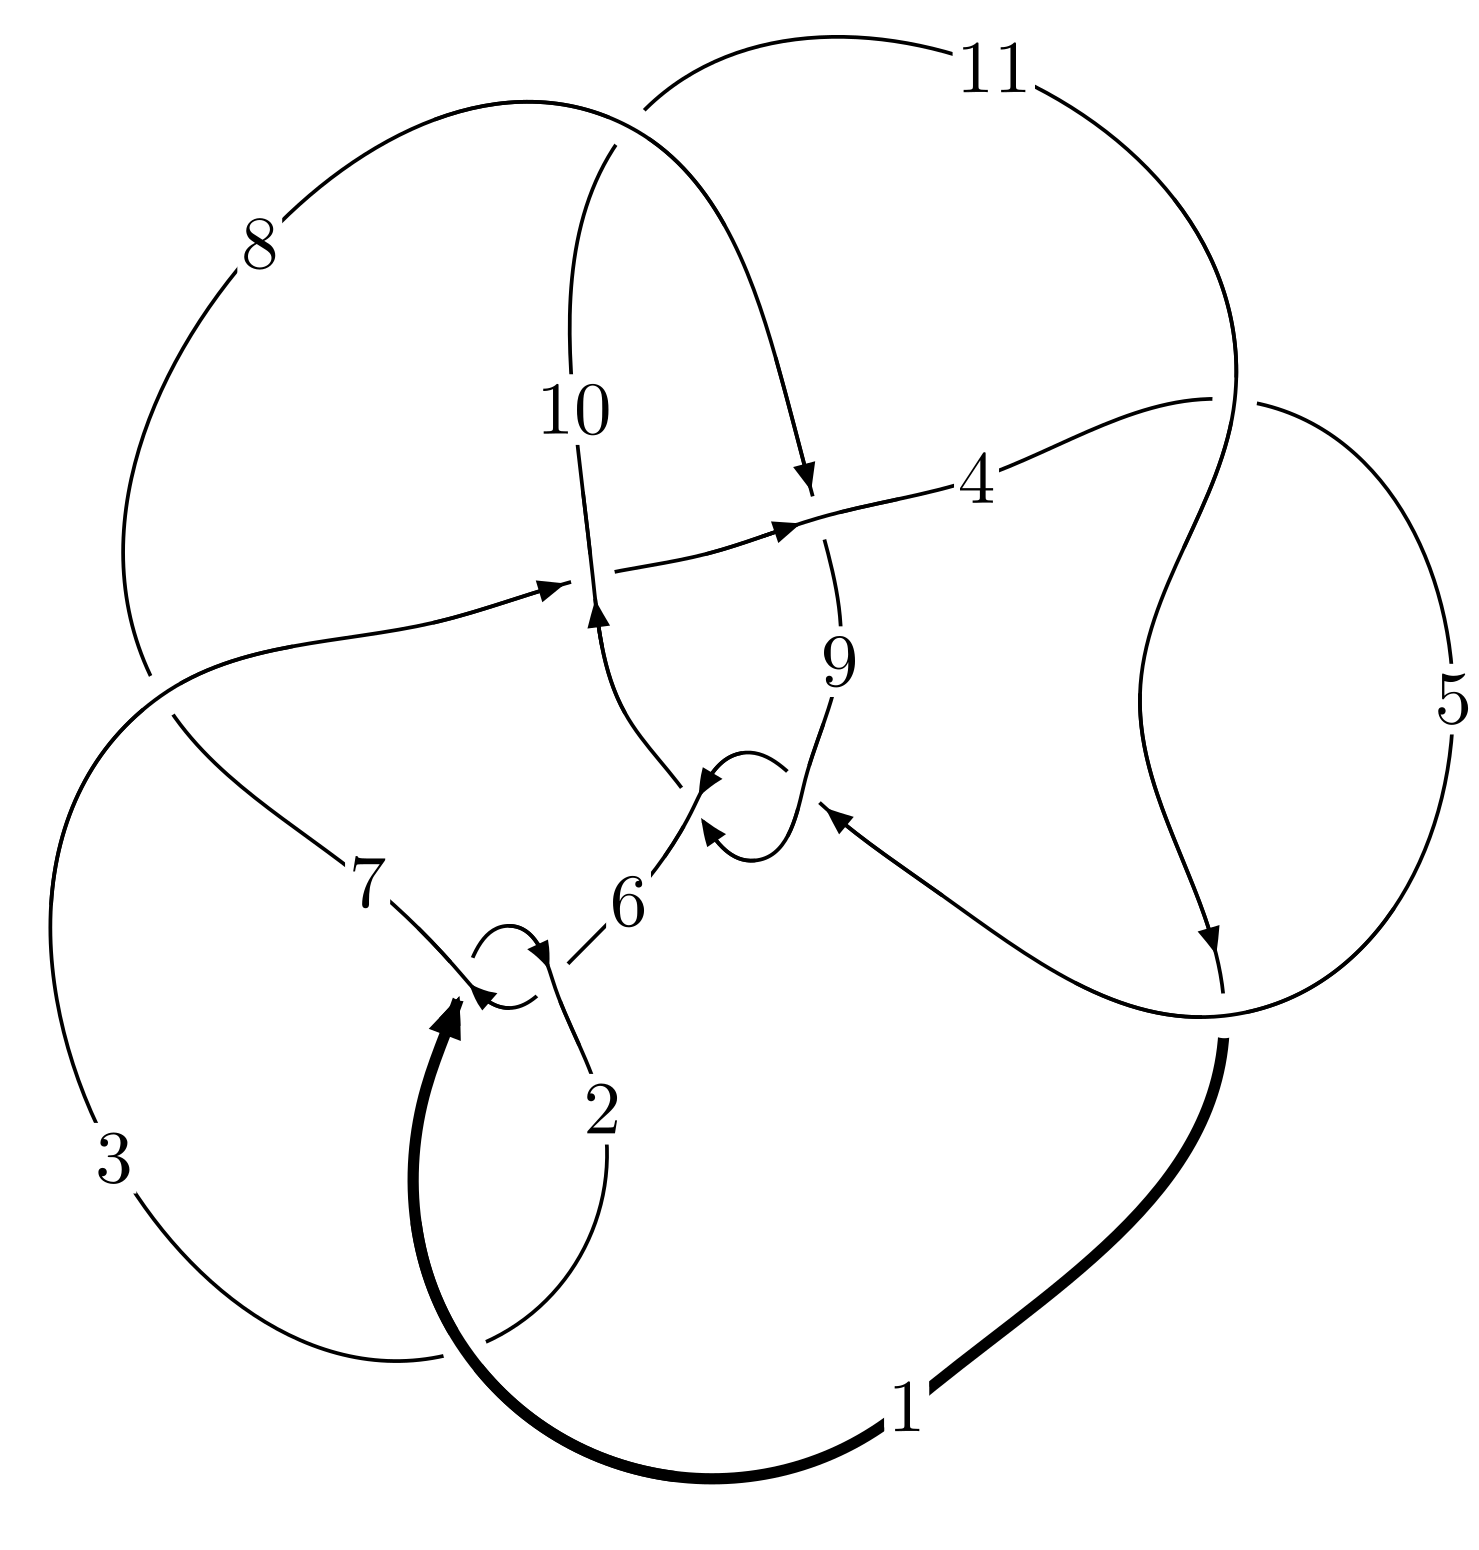
\includegraphics[width=112pt]{../../../GIT/diagram.site/Diagrams/png/438_11a_189.png}\\
\ \ \ A knot diagram\footnotemark}&
\allowdisplaybreaks
\textbf{Linearized knot diagam} \\
\cline{2-2}
 &
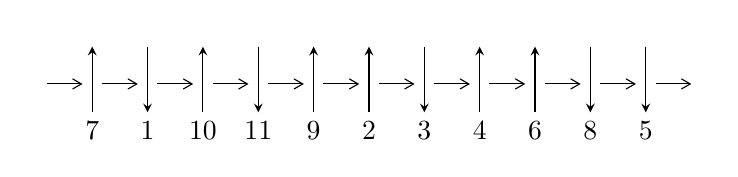
\begin{tikzpicture}[x=20pt, y=17pt]
	% nodes
	\node (C0) at (0, 0) {};
	\node (C1) at (1, 0) {};
	\node (C1U) at (1, +1) {};
	\node (C1D) at (1, -1) {7};

	\node (C2) at (2, 0) {};
	\node (C2U) at (2, +1) {};
	\node (C2D) at (2, -1) {1};

	\node (C3) at (3, 0) {};
	\node (C3U) at (3, +1) {};
	\node (C3D) at (3, -1) {10};

	\node (C4) at (4, 0) {};
	\node (C4U) at (4, +1) {};
	\node (C4D) at (4, -1) {11};

	\node (C5) at (5, 0) {};
	\node (C5U) at (5, +1) {};
	\node (C5D) at (5, -1) {9};

	\node (C6) at (6, 0) {};
	\node (C6U) at (6, +1) {};
	\node (C6D) at (6, -1) {2};

	\node (C7) at (7, 0) {};
	\node (C7U) at (7, +1) {};
	\node (C7D) at (7, -1) {3};

	\node (C8) at (8, 0) {};
	\node (C8U) at (8, +1) {};
	\node (C8D) at (8, -1) {4};

	\node (C9) at (9, 0) {};
	\node (C9U) at (9, +1) {};
	\node (C9D) at (9, -1) {6};

	\node (C10) at (10, 0) {};
	\node (C10U) at (10, +1) {};
	\node (C10D) at (10, -1) {8};

	\node (C11) at (11, 0) {};
	\node (C11U) at (11, +1) {};
	\node (C11D) at (11, -1) {5};
	\node (C12) at (12, 0) {};

	% arrows
	\draw[->,>={angle 60}]
	(C0) edge (C1) (C1) edge (C2) (C2) edge (C3) (C3) edge (C4) (C4) edge (C5) (C5) edge (C6) (C6) edge (C7) (C7) edge (C8) (C8) edge (C9) (C9) edge (C10) (C10) edge (C11) (C11) edge (C12) ;	\draw[->,>=stealth]
	(C1D) edge (C1U) (C2U) edge (C2D) (C3D) edge (C3U) (C4U) edge (C4D) (C5D) edge (C5U) (C6D) edge (C6U) (C7U) edge (C7D) (C8D) edge (C8U) (C9D) edge (C9U) (C10U) edge (C10D) (C11U) edge (C11D) ;
	\end{tikzpicture} \\
\hhline{~~} \\& 
\textbf{Solving Sequence} \\ \cline{2-2} 
 &
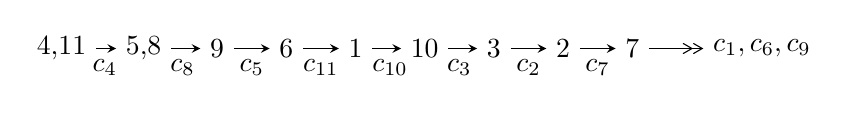
\begin{tikzpicture}[x=25pt, y=7pt]
	% node
	\node (A0) at (-1/8, 0) {4,11};
	\node (A1) at (17/16, 0) {5,8};
	\node (A2) at (17/8, 0) {9};
	\node (A3) at (25/8, 0) {6};
	\node (A4) at (33/8, 0) {1};
	\node (A5) at (41/8, 0) {10};
	\node (A6) at (49/8, 0) {3};
	\node (A7) at (57/8, 0) {2};
	\node (A8) at (65/8, 0) {7};
	\node (C1) at (1/2, -1) {$c_{4}$};
	\node (C2) at (13/8, -1) {$c_{8}$};
	\node (C3) at (21/8, -1) {$c_{5}$};
	\node (C4) at (29/8, -1) {$c_{11}$};
	\node (C5) at (37/8, -1) {$c_{10}$};
	\node (C6) at (45/8, -1) {$c_{3}$};
	\node (C7) at (53/8, -1) {$c_{2}$};
	\node (C8) at (61/8, -1) {$c_{7}$};
	\node (A9) at (10, 0) {$c_{1},c_{6},c_{9}$};

	% edge
	\draw[->,>=stealth]	
	(A0) edge (A1) (A1) edge (A2) (A2) edge (A3) (A3) edge (A4) (A4) edge (A5) (A5) edge (A6) (A6) edge (A7) (A7) edge (A8) ;
	\draw[->>,>={angle 60}]	
	(A8) edge (A9);
\end{tikzpicture} \\ 

\end{tabular} \\

\footnotetext{
The image of knot diagram is generated by the software ``\textbf{Draw programme}" developed by Andrew Bartholomew(\url{http://www.layer8.co.uk/maths/draw/index.htm\#Running-draw}), where we modified some parts for our purpose(\url{https://github.com/CATsTAILs/LinksPainter}).
}\phantom \\ \newline 
\centering \textbf{Ideals for irreducible components\footnotemark of $X_{\text{par}}$} 
 
\begin{align*}
I^u_{1}&=\langle 
6.42009\times10^{257} u^{88}-4.87876\times10^{257} u^{87}+\cdots+2.36068\times10^{257} b+8.83509\times10^{259},\\
\phantom{I^u_{1}}&\phantom{= \langle  }6.20222\times10^{258} u^{88}+4.18516\times10^{258} u^{87}+\cdots+3.09249\times10^{259} a+2.68994\times10^{260},\\
\phantom{I^u_{1}}&\phantom{= \langle  }u^{89}-30 u^{87}+\cdots-598 u+131\rangle \\
I^u_{2}&=\langle 
- u^{14}+u^{13}+5 u^{12}-4 u^{11}-12 u^{10}+9 u^9+17 u^8-15 u^7-14 u^6+12 u^5+6 u^4-7 u^3- u^2+b,\\
\phantom{I^u_{2}}&\phantom{= \langle  }-7 u^{14}+6 u^{13}+\cdots+a+7,\\
\phantom{I^u_{2}}&\phantom{= \langle  }u^{15}- u^{14}-6 u^{13}+5 u^{12}+17 u^{11}-13 u^{10}-29 u^9+24 u^8+31 u^7-27 u^6-20 u^5+19 u^4+7 u^3-7 u^2- u+1\rangle \\
\\
\end{align*}
\raggedright * 2 irreducible components of $\dim_{\mathbb{C}}=0$, with total 104 representations.\\
\footnotetext{All coefficients of polynomials are rational numbers. But the coefficients are sometimes approximated in decimal forms when there is not enough margin.}
\newpage
\renewcommand{\arraystretch}{1}
\centering \section*{I. $I^u_{1}= \langle 6.42\times10^{257} u^{88}-4.88\times10^{257} u^{87}+\cdots+2.36\times10^{257} b+8.84\times10^{259},\;6.20\times10^{258} u^{88}+4.19\times10^{258} u^{87}+\cdots+3.09\times10^{259} a+2.69\times10^{260},\;u^{89}-30 u^{87}+\cdots-598 u+131 \rangle$}
\flushleft \textbf{(i) Arc colorings}\\
\begin{tabular}{m{7pt} m{180pt} m{7pt} m{180pt} }
\flushright $a_{4}=$&$\begin{pmatrix}1\\0\end{pmatrix}$ \\
\flushright $a_{11}=$&$\begin{pmatrix}0\\u\end{pmatrix}$ \\
\flushright $a_{5}=$&$\begin{pmatrix}1\\u^2\end{pmatrix}$ \\
\flushright $a_{8}=$&$\begin{pmatrix}-0.200557 u^{88}-0.135333 u^{87}+\cdots+189.917 u-8.69828\\-2.71959 u^{88}+2.06667 u^{87}+\cdots+2244.10 u-374.260\end{pmatrix}$ \\
\flushright $a_{9}=$&$\begin{pmatrix}-2.92015 u^{88}+1.93134 u^{87}+\cdots+2434.01 u-382.958\\-2.71959 u^{88}+2.06667 u^{87}+\cdots+2244.10 u-374.260\end{pmatrix}$ \\
\flushright $a_{6}=$&$\begin{pmatrix}2.84782 u^{88}-2.54786 u^{87}+\cdots-2839.07 u+510.136\\0.594470 u^{88}-0.409964 u^{87}+\cdots-776.183 u+135.349\end{pmatrix}$ \\
\flushright $a_{1}=$&$\begin{pmatrix}- u\\- u^3+u\end{pmatrix}$ \\
\flushright $a_{10}=$&$\begin{pmatrix}-3.69459 u^{88}+2.73242 u^{87}+\cdots+2749.91 u-445.177\\-0.851550 u^{88}+0.449332 u^{87}+\cdots+777.942 u-121.621\end{pmatrix}$ \\
\flushright $a_{3}=$&$\begin{pmatrix}-1.70941 u^{88}+1.84202 u^{87}+\cdots+1720.23 u-327.215\\0.0173264 u^{88}+0.0106093 u^{87}+\cdots+245.379 u-48.9621\end{pmatrix}$ \\
\flushright $a_{2}=$&$\begin{pmatrix}-1.77307 u^{88}+1.96142 u^{87}+\cdots+1963.93 u-375.540\\0.0672428 u^{88}-0.0641570 u^{87}+\cdots+81.4241 u-16.2786\end{pmatrix}$ \\
\flushright $a_{7}=$&$\begin{pmatrix}-0.967025 u^{88}+1.19947 u^{87}+\cdots+1231.97 u-237.907\\-0.376658 u^{88}+0.389535 u^{87}+\cdots+428.290 u-81.3056\end{pmatrix}$\\ \flushright $a_{7}=$&$\begin{pmatrix}-0.967025 u^{88}+1.19947 u^{87}+\cdots+1231.97 u-237.907\\-0.376658 u^{88}+0.389535 u^{87}+\cdots+428.290 u-81.3056\end{pmatrix}$\\&\end{tabular}
\flushleft \textbf{(ii) Obstruction class $= -1$}\\~\\
\flushleft \textbf{(iii) Cusp Shapes $= 0.125878 u^{88}-0.576729 u^{87}+\cdots-1166.86 u+242.988$}\\~\\
\newpage\renewcommand{\arraystretch}{1}
\flushleft \textbf{(iv) u-Polynomials at the component}\newline \\
\begin{tabular}{m{50pt}|m{274pt}}
Crossings & \hspace{64pt}u-Polynomials at each crossing \\
\hline $$\begin{aligned}c_{1},c_{6}\end{aligned}$$&$\begin{aligned}
&u^{89}+u^{88}+\cdots+u+1
\end{aligned}$\\
\hline $$\begin{aligned}c_{2}\end{aligned}$$&$\begin{aligned}
&u^{89}+45 u^{88}+\cdots-7 u-1
\end{aligned}$\\
\hline $$\begin{aligned}c_{3}\end{aligned}$$&$\begin{aligned}
&u^{89}-3 u^{88}+\cdots+27 u+1
\end{aligned}$\\
\hline $$\begin{aligned}c_{4},c_{11}\end{aligned}$$&$\begin{aligned}
&u^{89}-30 u^{87}+\cdots-598 u+131
\end{aligned}$\\
\hline $$\begin{aligned}c_{5},c_{9}\end{aligned}$$&$\begin{aligned}
&u^{89}-27 u^{87}+\cdots+2 u-1
\end{aligned}$\\
\hline $$\begin{aligned}c_{7}\end{aligned}$$&$\begin{aligned}
&u^{89}- u^{88}+\cdots-219 u+3737
\end{aligned}$\\
\hline $$\begin{aligned}c_{8}\end{aligned}$$&$\begin{aligned}
&u^{89}+u^{88}+\cdots-11 u+3
\end{aligned}$\\
\hline $$\begin{aligned}c_{10}\end{aligned}$$&$\begin{aligned}
&u^{89}-11 u^{88}+\cdots+2752 u-593
\end{aligned}$\\
\hline
\end{tabular}\\~\\
\newpage\renewcommand{\arraystretch}{1}
\flushleft \textbf{(v) Riley Polynomials at the component}\newline \\
\begin{tabular}{m{50pt}|m{274pt}}
Crossings & \hspace{64pt}Riley Polynomials at each crossing \\
\hline $$\begin{aligned}c_{1},c_{6}\end{aligned}$$&$\begin{aligned}
&y^{89}+45 y^{88}+\cdots-7 y-1
\end{aligned}$\\
\hline $$\begin{aligned}c_{2}\end{aligned}$$&$\begin{aligned}
&y^{89}+y^{88}+\cdots-39 y-1
\end{aligned}$\\
\hline $$\begin{aligned}c_{3}\end{aligned}$$&$\begin{aligned}
&y^{89}+3 y^{88}+\cdots+143 y-1
\end{aligned}$\\
\hline $$\begin{aligned}c_{4},c_{11}\end{aligned}$$&$\begin{aligned}
&y^{89}-60 y^{88}+\cdots+397166 y-17161
\end{aligned}$\\
\hline $$\begin{aligned}c_{5},c_{9}\end{aligned}$$&$\begin{aligned}
&y^{89}-54 y^{88}+\cdots+32 y-1
\end{aligned}$\\
\hline $$\begin{aligned}c_{7}\end{aligned}$$&$\begin{aligned}
&y^{89}-43 y^{88}+\cdots-186682455 y-13965169
\end{aligned}$\\
\hline $$\begin{aligned}c_{8}\end{aligned}$$&$\begin{aligned}
&y^{89}+5 y^{88}+\cdots+181 y-9
\end{aligned}$\\
\hline $$\begin{aligned}c_{10}\end{aligned}$$&$\begin{aligned}
&y^{89}-27 y^{88}+\cdots+8974170 y-351649
\end{aligned}$\\
\hline
\end{tabular}\\~\\
\newpage\flushleft \textbf{(vi) Complex Volumes and Cusp Shapes}
$$\begin{array}{c|c|c}  
\text{Solutions to }I^u_{1}& \I (\text{vol} + \sqrt{-1}CS) & \text{Cusp shape}\\
 \hline 
\begin{aligned}
u &= -0.889747 + 0.452384 I \\
a &= -0.53880 + 1.76232 I \\
b &= \phantom{-}0.477239 + 0.302395 I\end{aligned}
 & -0.63006 + 8.68382 I & \phantom{-0.000000 } 0 \\ \hline\begin{aligned}
u &= -0.889747 - 0.452384 I \\
a &= -0.53880 - 1.76232 I \\
b &= \phantom{-}0.477239 - 0.302395 I\end{aligned}
 & -0.63006 - 8.68382 I & \phantom{-0.000000 } 0 \\ \hline\begin{aligned}
u &= \phantom{-}0.910671 + 0.398320 I \\
a &= \phantom{-}0.19557 + 1.62064 I \\
b &= -0.403492 + 0.311347 I\end{aligned}
 & \phantom{-}1.47236 - 3.97526 I & \phantom{-0.000000 } 0 \\ \hline\begin{aligned}
u &= \phantom{-}0.910671 - 0.398320 I \\
a &= \phantom{-}0.19557 - 1.62064 I \\
b &= -0.403492 - 0.311347 I\end{aligned}
 & \phantom{-}1.47236 + 3.97526 I & \phantom{-0.000000 } 0 \\ \hline\begin{aligned}
u &= -1.016600 + 0.137245 I \\
a &= -0.576279 - 0.124219 I \\
b &= \phantom{-}1.28500 - 1.71908 I\end{aligned}
 & -0.83265 + 2.51437 I & \phantom{-0.000000 } 0 \\ \hline\begin{aligned}
u &= -1.016600 - 0.137245 I \\
a &= -0.576279 + 0.124219 I \\
b &= \phantom{-}1.28500 + 1.71908 I\end{aligned}
 & -0.83265 - 2.51437 I & \phantom{-0.000000 } 0 \\ \hline\begin{aligned}
u &= -0.954288 + 0.091707 I \\
a &= \phantom{-}1.90084 + 0.00472 I \\
b &= -1.231680 + 0.032158 I\end{aligned}
 & \phantom{-}0.74745 + 3.52422 I & \phantom{-0.000000 } 0 \\ \hline\begin{aligned}
u &= -0.954288 - 0.091707 I \\
a &= \phantom{-}1.90084 - 0.00472 I \\
b &= -1.231680 - 0.032158 I\end{aligned}
 & \phantom{-}0.74745 - 3.52422 I & \phantom{-0.000000 } 0 \\ \hline\begin{aligned}
u &= \phantom{-}0.912318 + 0.259542 I \\
a &= -0.65851 + 1.37947 I \\
b &= -0.259979 + 0.234024 I\end{aligned}
 & \phantom{-}2.10633 - 2.24661 I & \phantom{-0.000000 } 0 \\ \hline\begin{aligned}
u &= \phantom{-}0.912318 - 0.259542 I \\
a &= -0.65851 - 1.37947 I \\
b &= -0.259979 - 0.234024 I\end{aligned}
 & \phantom{-}2.10633 + 2.24661 I & \phantom{-0.000000 } 0\\
 \hline 
 \end{array}$$\newpage$$\begin{array}{c|c|c}  
\text{Solutions to }I^u_{1}& \I (\text{vol} + \sqrt{-1}CS) & \text{Cusp shape}\\
 \hline 
\begin{aligned}
u &= \phantom{-}0.250513 + 0.909541 I \\
a &= \phantom{-}0.558779 + 0.800837 I \\
b &= -1.012260 - 0.599113 I\end{aligned}
 & \phantom{-}5.28492 + 4.09985 I & \phantom{-0.000000 } 0 \\ \hline\begin{aligned}
u &= \phantom{-}0.250513 - 0.909541 I \\
a &= \phantom{-}0.558779 - 0.800837 I \\
b &= -1.012260 + 0.599113 I\end{aligned}
 & \phantom{-}5.28492 - 4.09985 I & \phantom{-0.000000 } 0 \\ \hline\begin{aligned}
u &= \phantom{-}1.061570 + 0.193566 I \\
a &= \phantom{-}0.646957 + 0.005889 I \\
b &= -1.34806 - 1.48412 I\end{aligned}
 & -3.38961 - 8.10177 I & \phantom{-0.000000 } 0 \\ \hline\begin{aligned}
u &= \phantom{-}1.061570 - 0.193566 I \\
a &= \phantom{-}0.646957 - 0.005889 I \\
b &= -1.34806 + 1.48412 I\end{aligned}
 & -3.38961 + 8.10177 I & \phantom{-0.000000 } 0 \\ \hline\begin{aligned}
u &= -0.896503 + 0.169355 I \\
a &= \phantom{-}1.19590 + 1.09495 I \\
b &= \phantom{-}0.204472 + 0.156620 I\end{aligned}
 & \phantom{-}0.70886 - 2.35289 I & \phantom{-0.000000 } 0 \\ \hline\begin{aligned}
u &= -0.896503 - 0.169355 I \\
a &= \phantom{-}1.19590 - 1.09495 I \\
b &= \phantom{-}0.204472 - 0.156620 I\end{aligned}
 & \phantom{-}0.70886 + 2.35289 I & \phantom{-0.000000 } 0 \\ \hline\begin{aligned}
u &= \phantom{-}1.096800 + 0.024032 I \\
a &= \phantom{-}0.843907 - 0.225610 I \\
b &= -0.97444 - 1.43273 I\end{aligned}
 & -6.30667 + 0.58881 I & \phantom{-0.000000 } 0 \\ \hline\begin{aligned}
u &= \phantom{-}1.096800 - 0.024032 I \\
a &= \phantom{-}0.843907 + 0.225610 I \\
b &= -0.97444 + 1.43273 I\end{aligned}
 & -6.30667 - 0.58881 I & \phantom{-0.000000 } 0 \\ \hline\begin{aligned}
u &= -0.593963 + 0.659935 I \\
a &= \phantom{-}0.857622 + 0.233636 I \\
b &= -0.639884 - 0.077817 I\end{aligned}
 & -0.74312 + 2.38513 I & \phantom{-0.000000 } 0 \\ \hline\begin{aligned}
u &= -0.593963 - 0.659935 I \\
a &= \phantom{-}0.857622 - 0.233636 I \\
b &= -0.639884 + 0.077817 I\end{aligned}
 & -0.74312 - 2.38513 I & \phantom{-0.000000 } 0\\
 \hline 
 \end{array}$$\newpage$$\begin{array}{c|c|c}  
\text{Solutions to }I^u_{1}& \I (\text{vol} + \sqrt{-1}CS) & \text{Cusp shape}\\
 \hline 
\begin{aligned}
u &= -1.018630 + 0.485863 I \\
a &= -0.760663 + 0.983882 I \\
b &= \phantom{-}0.506841 + 0.529809 I\end{aligned}
 & -2.24793 + 1.87180 I & \phantom{-0.000000 } 0 \\ \hline\begin{aligned}
u &= -1.018630 - 0.485863 I \\
a &= -0.760663 - 0.983882 I \\
b &= \phantom{-}0.506841 - 0.529809 I\end{aligned}
 & -2.24793 - 1.87180 I & \phantom{-0.000000 } 0 \\ \hline\begin{aligned}
u &= \phantom{-}0.398710 + 0.771706 I \\
a &= \phantom{-}1.354100 - 0.383086 I \\
b &= -0.449816 + 0.871067 I\end{aligned}
 & -2.27469 - 6.43119 I & \phantom{-0.000000 } 0 \\ \hline\begin{aligned}
u &= \phantom{-}0.398710 - 0.771706 I \\
a &= \phantom{-}1.354100 + 0.383086 I \\
b &= -0.449816 - 0.871067 I\end{aligned}
 & -2.27469 + 6.43119 I & \phantom{-0.000000 } 0 \\ \hline\begin{aligned}
u &= -0.651535 + 0.565177 I \\
a &= \phantom{-}1.57091 + 0.04849 I \\
b &= -1.016120 + 0.181206 I\end{aligned}
 & \phantom{-}0.03725 - 4.55071 I & \phantom{-0.000000 } 0 \\ \hline\begin{aligned}
u &= -0.651535 - 0.565177 I \\
a &= \phantom{-}1.57091 - 0.04849 I \\
b &= -1.016120 - 0.181206 I\end{aligned}
 & \phantom{-}0.03725 + 4.55071 I & \phantom{-0.000000 } 0 \\ \hline\begin{aligned}
u &= \phantom{-}1.080740 + 0.451595 I \\
a &= \phantom{-}1.089600 + 0.543941 I \\
b &= -0.652720 + 0.801813 I\end{aligned}
 & -1.82833 - 5.02044 I & \phantom{-0.000000 } 0 \\ \hline\begin{aligned}
u &= \phantom{-}1.080740 - 0.451595 I \\
a &= \phantom{-}1.089600 - 0.543941 I \\
b &= -0.652720 - 0.801813 I\end{aligned}
 & -1.82833 + 5.02044 I & \phantom{-0.000000 } 0 \\ \hline\begin{aligned}
u &= \phantom{-}0.825079 + 0.852973 I \\
a &= \phantom{-}1.013710 - 0.231765 I \\
b &= -0.404411 + 0.990807 I\end{aligned}
 & -2.85121 + 0.37716 I & \phantom{-0.000000 } 0 \\ \hline\begin{aligned}
u &= \phantom{-}0.825079 - 0.852973 I \\
a &= \phantom{-}1.013710 + 0.231765 I \\
b &= -0.404411 - 0.990807 I\end{aligned}
 & -2.85121 - 0.37716 I & \phantom{-0.000000 } 0\\
 \hline 
 \end{array}$$\newpage$$\begin{array}{c|c|c}  
\text{Solutions to }I^u_{1}& \I (\text{vol} + \sqrt{-1}CS) & \text{Cusp shape}\\
 \hline 
\begin{aligned}
u &= -0.799407 + 0.019558 I \\
a &= -0.815403 - 0.950050 I \\
b &= \phantom{-}0.20638 - 1.47781 I\end{aligned}
 & \phantom{-}0.082135 - 1.402700 I & \phantom{-}1.000000 + 0.911438 I \\ \hline\begin{aligned}
u &= -0.799407 - 0.019558 I \\
a &= -0.815403 + 0.950050 I \\
b &= \phantom{-}0.20638 + 1.47781 I\end{aligned}
 & \phantom{-}0.082135 + 1.402700 I & \phantom{-}1.000000 - 0.911438 I \\ \hline\begin{aligned}
u &= \phantom{-}0.127992 + 1.209710 I \\
a &= \phantom{-}0.551795 + 0.738924 I \\
b &= -0.807284 - 0.641410 I\end{aligned}
 & \phantom{-}2.99214 + 5.76178 I & \phantom{-0.000000 } 0 \\ \hline\begin{aligned}
u &= \phantom{-}0.127992 - 1.209710 I \\
a &= \phantom{-}0.551795 - 0.738924 I \\
b &= -0.807284 + 0.641410 I\end{aligned}
 & \phantom{-}2.99214 - 5.76178 I & \phantom{-0.000000 } 0 \\ \hline\begin{aligned}
u &= \phantom{-}0.758651 + 0.141414 I \\
a &= -1.92316 + 0.06017 I \\
b &= \phantom{-}1.166660 + 0.036708 I\end{aligned}
 & \phantom{-}2.87128 + 0.16130 I & \phantom{-}2.26530 + 3.31981 I \\ \hline\begin{aligned}
u &= \phantom{-}0.758651 - 0.141414 I \\
a &= -1.92316 - 0.06017 I \\
b &= \phantom{-}1.166660 - 0.036708 I\end{aligned}
 & \phantom{-}2.87128 - 0.16130 I & \phantom{-}2.26530 - 3.31981 I \\ \hline\begin{aligned}
u &= \phantom{-}0.049165 + 1.230130 I \\
a &= -0.559202 + 0.688042 I \\
b &= \phantom{-}0.736512 - 0.561358 I\end{aligned}
 & -1.33196 - 2.44177 I & \phantom{-0.000000 } 0 \\ \hline\begin{aligned}
u &= \phantom{-}0.049165 - 1.230130 I \\
a &= -0.559202 - 0.688042 I \\
b &= \phantom{-}0.736512 + 0.561358 I\end{aligned}
 & -1.33196 + 2.44177 I & \phantom{-0.000000 } 0 \\ \hline\begin{aligned}
u &= -0.305027 + 0.698562 I \\
a &= -0.476739 + 0.863083 I \\
b &= \phantom{-}1.162640 - 0.546817 I\end{aligned}
 & \phantom{-}4.93245 + 0.64307 I & \phantom{-}7.39513 - 2.13919 I \\ \hline\begin{aligned}
u &= -0.305027 - 0.698562 I \\
a &= -0.476739 - 0.863083 I \\
b &= \phantom{-}1.162640 + 0.546817 I\end{aligned}
 & \phantom{-}4.93245 - 0.64307 I & \phantom{-}7.39513 + 2.13919 I\\
 \hline 
 \end{array}$$\newpage$$\begin{array}{c|c|c}  
\text{Solutions to }I^u_{1}& \I (\text{vol} + \sqrt{-1}CS) & \text{Cusp shape}\\
 \hline 
\begin{aligned}
u &= -0.439575 + 0.615498 I \\
a &= \phantom{-}1.149600 - 0.115471 I \\
b &= -0.698187 + 0.241172 I\end{aligned}
 & -0.66030 + 2.49036 I & \phantom{-}1.19350 - 2.71078 I \\ \hline\begin{aligned}
u &= -0.439575 - 0.615498 I \\
a &= \phantom{-}1.149600 + 0.115471 I \\
b &= -0.698187 - 0.241172 I\end{aligned}
 & -0.66030 - 2.49036 I & \phantom{-}1.19350 + 2.71078 I \\ \hline\begin{aligned}
u &= -1.178450 + 0.416595 I \\
a &= \phantom{-}0.747568 - 0.419084 I \\
b &= -1.21853 - 1.36797 I\end{aligned}
 & \phantom{-}2.16092 + 3.60298 I & \phantom{-0.000000 } 0 \\ \hline\begin{aligned}
u &= -1.178450 - 0.416595 I \\
a &= \phantom{-}0.747568 + 0.419084 I \\
b &= -1.21853 + 1.36797 I\end{aligned}
 & \phantom{-}2.16092 - 3.60298 I & \phantom{-0.000000 } 0 \\ \hline\begin{aligned}
u &= -1.216440 + 0.411059 I \\
a &= -0.122681 + 0.284283 I \\
b &= \phantom{-}0.107118 + 0.672929 I\end{aligned}
 & -2.06773 + 2.36101 I & \phantom{-0.000000 } 0 \\ \hline\begin{aligned}
u &= -1.216440 - 0.411059 I \\
a &= -0.122681 - 0.284283 I \\
b &= \phantom{-}0.107118 - 0.672929 I\end{aligned}
 & -2.06773 - 2.36101 I & \phantom{-0.000000 } 0 \\ \hline\begin{aligned}
u &= \phantom{-}1.234760 + 0.357842 I \\
a &= \phantom{-}1.253570 + 0.379206 I \\
b &= -0.889269 + 0.916124 I\end{aligned}
 & -4.17367 - 5.52755 I & \phantom{-0.000000 } 0 \\ \hline\begin{aligned}
u &= \phantom{-}1.234760 - 0.357842 I \\
a &= \phantom{-}1.253570 - 0.379206 I \\
b &= -0.889269 - 0.916124 I\end{aligned}
 & -4.17367 + 5.52755 I & \phantom{-0.000000 } 0 \\ \hline\begin{aligned}
u &= -1.262070 + 0.281444 I \\
a &= -1.224250 + 0.302827 I \\
b &= \phantom{-}0.931584 + 0.992768 I\end{aligned}
 & -8.23912 + 1.98284 I & \phantom{-0.000000 } 0 \\ \hline\begin{aligned}
u &= -1.262070 - 0.281444 I \\
a &= -1.224250 - 0.302827 I \\
b &= \phantom{-}0.931584 - 0.992768 I\end{aligned}
 & -8.23912 - 1.98284 I & \phantom{-0.000000 } 0\\
 \hline 
 \end{array}$$\newpage$$\begin{array}{c|c|c}  
\text{Solutions to }I^u_{1}& \I (\text{vol} + \sqrt{-1}CS) & \text{Cusp shape}\\
 \hline 
\begin{aligned}
u &= -1.036670 + 0.779876 I \\
a &= -0.780160 - 0.133305 I \\
b &= \phantom{-}0.327917 + 0.979792 I\end{aligned}
 & -1.06082 + 3.18631 I & \phantom{-0.000000 } 0 \\ \hline\begin{aligned}
u &= -1.036670 - 0.779876 I \\
a &= -0.780160 + 0.133305 I \\
b &= \phantom{-}0.327917 - 0.979792 I\end{aligned}
 & -1.06082 - 3.18631 I & \phantom{-0.000000 } 0 \\ \hline\begin{aligned}
u &= \phantom{-}0.552589 + 0.430106 I \\
a &= -1.64524 + 0.28442 I \\
b &= \phantom{-}1.032220 + 0.058574 I\end{aligned}
 & \phantom{-}2.41961 + 0.34900 I & \phantom{-}5.67559 + 0.69336 I \\ \hline\begin{aligned}
u &= \phantom{-}0.552589 - 0.430106 I \\
a &= -1.64524 - 0.28442 I \\
b &= \phantom{-}1.032220 - 0.058574 I\end{aligned}
 & \phantom{-}2.41961 - 0.34900 I & \phantom{-}5.67559 - 0.69336 I \\ \hline\begin{aligned}
u &= -0.148725 + 1.301670 I \\
a &= -0.530595 + 0.740434 I \\
b &= \phantom{-}0.767567 - 0.682700 I\end{aligned}
 & \phantom{-}0.33138 - 10.71180 I & \phantom{-0.000000 } 0 \\ \hline\begin{aligned}
u &= -0.148725 - 1.301670 I \\
a &= -0.530595 - 0.740434 I \\
b &= \phantom{-}0.767567 + 0.682700 I\end{aligned}
 & \phantom{-}0.33138 + 10.71180 I & \phantom{-0.000000 } 0 \\ \hline\begin{aligned}
u &= \phantom{-}1.220660 + 0.503248 I \\
a &= -0.890977 - 0.373556 I \\
b &= \phantom{-}1.15837 - 1.27935 I\end{aligned}
 & \phantom{-}2.20718 - 9.21559 I & \phantom{-0.000000 } 0 \\ \hline\begin{aligned}
u &= \phantom{-}1.220660 - 0.503248 I \\
a &= -0.890977 + 0.373556 I \\
b &= \phantom{-}1.15837 + 1.27935 I\end{aligned}
 & \phantom{-}2.20718 + 9.21559 I & \phantom{-0.000000 } 0 \\ \hline\begin{aligned}
u &= -1.32135\phantom{ +0.000000I} \\
a &= \phantom{-}0.470030\phantom{ +0.000000I} \\
b &= -1.92284\phantom{ +0.000000I}\end{aligned}
 & -3.01024\phantom{ +0.000000I} & \phantom{-0.000000 } 0 \\ \hline\begin{aligned}
u &= -1.282490 + 0.377633 I \\
a &= -1.306930 + 0.361809 I \\
b &= \phantom{-}0.939471 + 0.891330 I\end{aligned}
 & -6.96009 + 10.29770 I & \phantom{-0.000000 } 0\\
 \hline 
 \end{array}$$\newpage$$\begin{array}{c|c|c}  
\text{Solutions to }I^u_{1}& \I (\text{vol} + \sqrt{-1}CS) & \text{Cusp shape}\\
 \hline 
\begin{aligned}
u &= -1.282490 - 0.377633 I \\
a &= -1.306930 - 0.361809 I \\
b &= \phantom{-}0.939471 - 0.891330 I\end{aligned}
 & -6.96009 - 10.29770 I & \phantom{-0.000000 } 0 \\ \hline\begin{aligned}
u &= -0.230086 + 0.571128 I \\
a &= -1.52959 - 0.58458 I \\
b &= \phantom{-}0.360119 + 0.766641 I\end{aligned}
 & -0.07957 + 2.04453 I & \phantom{-}1.68178 - 3.11842 I \\ \hline\begin{aligned}
u &= -0.230086 - 0.571128 I \\
a &= -1.52959 + 0.58458 I \\
b &= \phantom{-}0.360119 - 0.766641 I\end{aligned}
 & -0.07957 - 2.04453 I & \phantom{-}1.68178 + 3.11842 I \\ \hline\begin{aligned}
u &= \phantom{-}0.603771 + 0.027652 I \\
a &= \phantom{-}1.30220 - 1.60314 I \\
b &= -0.026312 - 1.201250 I\end{aligned}
 & -1.77198 + 6.54158 I & -1.95190 - 4.07828 I \\ \hline\begin{aligned}
u &= \phantom{-}0.603771 - 0.027652 I \\
a &= \phantom{-}1.30220 + 1.60314 I \\
b &= -0.026312 + 1.201250 I\end{aligned}
 & -1.77198 - 6.54158 I & -1.95190 + 4.07828 I \\ \hline\begin{aligned}
u &= \phantom{-}1.41437 + 0.17024 I \\
a &= -0.578378 - 0.040899 I \\
b &= \phantom{-}1.37461 - 0.73147 I\end{aligned}
 & -7.33407 - 4.81411 I & \phantom{-0.000000 } 0 \\ \hline\begin{aligned}
u &= \phantom{-}1.41437 - 0.17024 I \\
a &= -0.578378 + 0.040899 I \\
b &= \phantom{-}1.37461 + 0.73147 I\end{aligned}
 & -7.33407 + 4.81411 I & \phantom{-0.000000 } 0 \\ \hline\begin{aligned}
u &= \phantom{-}0.131343 + 0.540464 I \\
a &= -1.041380 - 0.558162 I \\
b &= \phantom{-}0.427017 + 0.464554 I\end{aligned}
 & \phantom{-}0.725380 + 1.180740 I & \phantom{-}4.24551 - 4.64635 I \\ \hline\begin{aligned}
u &= \phantom{-}0.131343 - 0.540464 I \\
a &= -1.041380 + 0.558162 I \\
b &= \phantom{-}0.427017 - 0.464554 I\end{aligned}
 & \phantom{-}0.725380 - 1.180740 I & \phantom{-}4.24551 + 4.64635 I \\ \hline\begin{aligned}
u &= -1.24203 + 0.75104 I \\
a &= -0.513911 - 0.174215 I \\
b &= \phantom{-}0.208309 + 0.988394 I\end{aligned}
 & -1.64043 + 3.35164 I & \phantom{-0.000000 } 0\\
 \hline 
 \end{array}$$\newpage$$\begin{array}{c|c|c}  
\text{Solutions to }I^u_{1}& \I (\text{vol} + \sqrt{-1}CS) & \text{Cusp shape}\\
 \hline 
\begin{aligned}
u &= -1.24203 - 0.75104 I \\
a &= -0.513911 + 0.174215 I \\
b &= \phantom{-}0.208309 - 0.988394 I\end{aligned}
 & -1.64043 - 3.35164 I & \phantom{-0.000000 } 0 \\ \hline\begin{aligned}
u &= -1.46335 + 0.12164 I \\
a &= \phantom{-}0.480507 + 0.020198 I \\
b &= -0.528818 - 0.273350 I\end{aligned}
 & -3.43024 + 0.04199 I & \phantom{-0.000000 } 0 \\ \hline\begin{aligned}
u &= -1.46335 - 0.12164 I \\
a &= \phantom{-}0.480507 - 0.020198 I \\
b &= -0.528818 + 0.273350 I\end{aligned}
 & -3.43024 - 0.04199 I & \phantom{-0.000000 } 0 \\ \hline\begin{aligned}
u &= \phantom{-}1.34178 + 0.60423 I \\
a &= -1.029560 - 0.209600 I \\
b &= \phantom{-}1.12935 - 1.20094 I\end{aligned}
 & -0.85217 - 12.06680 I & \phantom{-0.000000 } 0 \\ \hline\begin{aligned}
u &= \phantom{-}1.34178 - 0.60423 I \\
a &= -1.029560 + 0.209600 I \\
b &= \phantom{-}1.12935 + 1.20094 I\end{aligned}
 & -0.85217 + 12.06680 I & \phantom{-0.000000 } 0 \\ \hline\begin{aligned}
u &= -1.38287 + 0.55098 I \\
a &= \phantom{-}0.963569 - 0.160924 I \\
b &= -1.14535 - 1.18423 I\end{aligned}
 & -5.82286 + 8.54509 I & \phantom{-0.000000 } 0 \\ \hline\begin{aligned}
u &= -1.38287 - 0.55098 I \\
a &= \phantom{-}0.963569 + 0.160924 I \\
b &= -1.14535 + 1.18423 I\end{aligned}
 & -5.82286 - 8.54509 I & \phantom{-0.000000 } 0 \\ \hline\begin{aligned}
u &= -1.36397 + 0.63423 I \\
a &= \phantom{-}1.064370 - 0.179821 I \\
b &= -1.12193 - 1.19463 I\end{aligned}
 & -3.5526 + 17.3742 I & \phantom{-0.000000 } 0 \\ \hline\begin{aligned}
u &= -1.36397 - 0.63423 I \\
a &= \phantom{-}1.064370 + 0.179821 I \\
b &= -1.12193 + 1.19463 I\end{aligned}
 & -3.5526 - 17.3742 I & \phantom{-0.000000 } 0 \\ \hline\begin{aligned}
u &= \phantom{-}1.51493 + 0.02764 I \\
a &= -0.466561 + 0.057922 I \\
b &= \phantom{-}0.646933 - 0.507679 I\end{aligned}
 & -6.87250 + 4.47387 I & \phantom{-0.000000 } 0\\
 \hline 
 \end{array}$$\newpage$$\begin{array}{c|c|c}  
\text{Solutions to }I^u_{1}& \I (\text{vol} + \sqrt{-1}CS) & \text{Cusp shape}\\
 \hline 
\begin{aligned}
u &= \phantom{-}1.51493 - 0.02764 I \\
a &= -0.466561 - 0.057922 I \\
b &= \phantom{-}0.646933 + 0.507679 I\end{aligned}
 & -6.87250 - 4.47387 I & \phantom{-0.000000 } 0 \\ \hline\begin{aligned}
u &= \phantom{-}1.38354 + 0.69467 I \\
a &= \phantom{-}0.327847 - 0.218814 I \\
b &= -0.099863 + 0.997213 I\end{aligned}
 & -4.70888 + 0.05763 I & \phantom{-0.000000 } 0 \\ \hline\begin{aligned}
u &= \phantom{-}1.38354 - 0.69467 I \\
a &= \phantom{-}0.327847 + 0.218814 I \\
b &= -0.099863 - 0.997213 I\end{aligned}
 & -4.70888 - 0.05763 I & \phantom{-0.000000 } 0 \\ \hline\begin{aligned}
u &= \phantom{-}1.32097 + 0.83036 I \\
a &= \phantom{-}0.479237 - 0.302029 I \\
b &= -0.183639 + 1.056270 I\end{aligned}
 & -4.21471 - 7.50514 I & \phantom{-0.000000 } 0 \\ \hline\begin{aligned}
u &= \phantom{-}1.32097 - 0.83036 I \\
a &= \phantom{-}0.479237 + 0.302029 I \\
b &= -0.183639 - 1.056270 I\end{aligned}
 & -4.21471 + 7.50514 I & \phantom{-0.000000 } 0 \\ \hline\begin{aligned}
u &= \phantom{-}1.64763 + 0.24323 I \\
a &= -0.462216 + 0.038991 I \\
b &= \phantom{-}0.502599 - 0.125500 I\end{aligned}
 & -7.01352 - 4.49963 I & \phantom{-0.000000 } 0 \\ \hline\begin{aligned}
u &= \phantom{-}1.64763 - 0.24323 I \\
a &= -0.462216 - 0.038991 I \\
b &= \phantom{-}0.502599 + 0.125500 I\end{aligned}
 & -7.01352 + 4.49963 I & \phantom{-0.000000 } 0 \\ \hline\begin{aligned}
u &= \phantom{-}0.194550 + 0.184951 I \\
a &= \phantom{-}4.04115 - 1.45822 I \\
b &= -0.085459 + 0.814007 I\end{aligned}
 & -3.77027 + 0.40204 I & -7.60841 - 1.19387 I \\ \hline\begin{aligned}
u &= \phantom{-}0.194550 - 0.184951 I \\
a &= \phantom{-}4.04115 + 1.45822 I \\
b &= -0.085459 - 0.814007 I\end{aligned}
 & -3.77027 - 0.40204 I & -7.60841 + 1.19387 I\\
 \hline 
 \end{array}$$\newpage\newpage\renewcommand{\arraystretch}{1}
\centering \section*{II. $I^u_{2}= \langle - u^{14}+u^{13}+\cdots- u^2+b,\;-7 u^{14}+6 u^{13}+\cdots+a+7,\;u^{15}- u^{14}+\cdots- u+1 \rangle$}
\flushleft \textbf{(i) Arc colorings}\\
\begin{tabular}{m{7pt} m{180pt} m{7pt} m{180pt} }
\flushright $a_{4}=$&$\begin{pmatrix}1\\0\end{pmatrix}$ \\
\flushright $a_{11}=$&$\begin{pmatrix}0\\u\end{pmatrix}$ \\
\flushright $a_{5}=$&$\begin{pmatrix}1\\u^2\end{pmatrix}$ \\
\flushright $a_{8}=$&$\begin{pmatrix}7 u^{14}-6 u^{13}+\cdots-23 u-7\\u^{14}- u^{13}+\cdots+7 u^3+u^2\end{pmatrix}$ \\
\flushright $a_{9}=$&$\begin{pmatrix}8 u^{14}-7 u^{13}+\cdots-23 u-7\\u^{14}- u^{13}+\cdots+7 u^3+u^2\end{pmatrix}$ \\
\flushright $a_{6}=$&$\begin{pmatrix}-7 u^{14}- u^{13}+\cdots-142 u^2+31\\- u^{13}+u^{12}+\cdots-6 u^2- u\end{pmatrix}$ \\
\flushright $a_{1}=$&$\begin{pmatrix}- u\\- u^3+u\end{pmatrix}$ \\
\flushright $a_{10}=$&$\begin{pmatrix}-23 u^{14}+17 u^{13}+\cdots+52 u+24\\u^{14}- u^{13}+\cdots-6 u-1\end{pmatrix}$ \\
\flushright $a_{3}=$&$\begin{pmatrix}18 u^{14}- u^{13}+\cdots-8 u-52\\- u^{14}+7 u^{12}+\cdots-25 u^2+6\end{pmatrix}$ \\
\flushright $a_{2}=$&$\begin{pmatrix}22 u^{14}- u^{13}+\cdots-9 u-63\\-4 u^{14}+27 u^{12}+\cdots+u+13\end{pmatrix}$ \\
\flushright $a_{7}=$&$\begin{pmatrix}-37 u^{14}+15 u^{13}+\cdots+32 u+61\\12 u^{14}-8 u^{13}+\cdots-17 u-12\end{pmatrix}$\\ \flushright $a_{7}=$&$\begin{pmatrix}-37 u^{14}+15 u^{13}+\cdots+32 u+61\\12 u^{14}-8 u^{13}+\cdots-17 u-12\end{pmatrix}$\\&\end{tabular}
\flushleft \textbf{(ii) Obstruction class $= 1$}\\~\\
\flushleft \textbf{(iii) Cusp Shapes $= -50 u^{14}+49 u^{13}+284 u^{12}-223 u^{11}-761 u^{10}+533 u^9+1213 u^8-928 u^7-1180 u^6+910 u^5+666 u^4-532 u^3-178 u^2+116 u+19$}\\~\\
\newpage\renewcommand{\arraystretch}{1}
\flushleft \textbf{(iv) u-Polynomials at the component}\newline \\
\begin{tabular}{m{50pt}|m{274pt}}
Crossings & \hspace{64pt}u-Polynomials at each crossing \\
\hline $$\begin{aligned}c_{1}\end{aligned}$$&$\begin{aligned}
&u^{15}+4 u^{13}+8 u^{11}- u^{10}+8 u^9-3 u^8+4 u^7-5 u^6-5 u^4-3 u^2-1
\end{aligned}$\\
\hline $$\begin{aligned}c_{2}\end{aligned}$$&$\begin{aligned}
&u^{15}+8 u^{14}+\cdots-6 u-1
\end{aligned}$\\
\hline $$\begin{aligned}c_{3}\end{aligned}$$&$\begin{aligned}
&u^{15}+u^{13}- u^{12}-2 u^{11}-2 u^9+4 u^8+2 u^7+u^5-4 u^4+1
\end{aligned}$\\
\hline $$\begin{aligned}c_{4}\end{aligned}$$&$\begin{aligned}
&u^{15}- u^{14}+\cdots- u+1
\end{aligned}$\\
\hline $$\begin{aligned}c_{5}\end{aligned}$$&$\begin{aligned}
&u^{15}- u^{14}+\cdots- u+1
\end{aligned}$\\
\hline $$\begin{aligned}c_{6}\end{aligned}$$&$\begin{aligned}
&u^{15}+4 u^{13}+8 u^{11}+u^{10}+8 u^9+3 u^8+4 u^7+5 u^6+5 u^4+3 u^2+1
\end{aligned}$\\
\hline $$\begin{aligned}c_{7}\end{aligned}$$&$\begin{aligned}
&u^{15}-4 u^{13}+\cdots+2 u+1
\end{aligned}$\\
\hline $$\begin{aligned}c_{8}\end{aligned}$$&$\begin{aligned}
&u^{15}-4 u^{11}+u^{10}+2 u^8+4 u^7-2 u^6-2 u^4- u^3+u^2+1
\end{aligned}$\\
\hline $$\begin{aligned}c_{9}\end{aligned}$$&$\begin{aligned}
&u^{15}+u^{14}+\cdots- u-1
\end{aligned}$\\
\hline $$\begin{aligned}c_{10}\end{aligned}$$&$\begin{aligned}
&u^{15}-4 u^{13}+\cdots+7 u+1
\end{aligned}$\\
\hline $$\begin{aligned}c_{11}\end{aligned}$$&$\begin{aligned}
&u^{15}+u^{14}+\cdots- u-1
\end{aligned}$\\
\hline
\end{tabular}\\~\\
\newpage\renewcommand{\arraystretch}{1}
\flushleft \textbf{(v) Riley Polynomials at the component}\newline \\
\begin{tabular}{m{50pt}|m{274pt}}
Crossings & \hspace{64pt}Riley Polynomials at each crossing \\
\hline $$\begin{aligned}c_{1},c_{6}\end{aligned}$$&$\begin{aligned}
&y^{15}+8 y^{14}+\cdots-6 y-1
\end{aligned}$\\
\hline $$\begin{aligned}c_{2}\end{aligned}$$&$\begin{aligned}
&y^{15}+16 y^{13}+\cdots-2 y-1
\end{aligned}$\\
\hline $$\begin{aligned}c_{3}\end{aligned}$$&$\begin{aligned}
&y^{15}+2 y^{14}+\cdots+8 y^2-1
\end{aligned}$\\
\hline $$\begin{aligned}c_{4},c_{11}\end{aligned}$$&$\begin{aligned}
&y^{15}-13 y^{14}+\cdots+15 y-1
\end{aligned}$\\
\hline $$\begin{aligned}c_{5},c_{9}\end{aligned}$$&$\begin{aligned}
&y^{15}-15 y^{14}+\cdots+13 y-1
\end{aligned}$\\
\hline $$\begin{aligned}c_{7}\end{aligned}$$&$\begin{aligned}
&y^{15}-8 y^{14}+\cdots-10 y-1
\end{aligned}$\\
\hline $$\begin{aligned}c_{8}\end{aligned}$$&$\begin{aligned}
&y^{15}-8 y^{13}+\cdots-2 y-1
\end{aligned}$\\
\hline $$\begin{aligned}c_{10}\end{aligned}$$&$\begin{aligned}
&y^{15}-8 y^{14}+\cdots+7 y-1
\end{aligned}$\\
\hline
\end{tabular}\\~\\
\newpage\flushleft \textbf{(vi) Complex Volumes and Cusp Shapes}
$$\begin{array}{c|c|c}  
\text{Solutions to }I^u_{2}& \I (\text{vol} + \sqrt{-1}CS) & \text{Cusp shape}\\
 \hline 
\begin{aligned}
u &= -0.906864 + 0.375829 I \\
a &= -0.537067 + 0.586861 I \\
b &= -0.058211 + 1.303160 I\end{aligned}
 & \phantom{-}0.29078 + 2.83345 I & \phantom{-}2.46812 - 4.57300 I \\ \hline\begin{aligned}
u &= -0.906864 - 0.375829 I \\
a &= -0.537067 - 0.586861 I \\
b &= -0.058211 - 1.303160 I\end{aligned}
 & \phantom{-}0.29078 - 2.83345 I & \phantom{-}2.46812 + 4.57300 I \\ \hline\begin{aligned}
u &= \phantom{-}0.786429 + 0.437105 I \\
a &= \phantom{-}0.904328 + 0.831344 I \\
b &= \phantom{-}0.187116 + 0.988050 I\end{aligned}
 & -1.62575 - 7.79387 I & -1.04019 + 8.56161 I \\ \hline\begin{aligned}
u &= \phantom{-}0.786429 - 0.437105 I \\
a &= \phantom{-}0.904328 - 0.831344 I \\
b &= \phantom{-}0.187116 - 0.988050 I\end{aligned}
 & -1.62575 + 7.79387 I & -1.04019 - 8.56161 I \\ \hline\begin{aligned}
u &= \phantom{-}0.878542 + 0.674122 I \\
a &= \phantom{-}0.998231 + 0.130624 I \\
b &= -0.106366 + 0.803002 I\end{aligned}
 & -3.32177 - 0.98994 I & -4.43129 + 2.79552 I \\ \hline\begin{aligned}
u &= \phantom{-}0.878542 - 0.674122 I \\
a &= \phantom{-}0.998231 - 0.130624 I \\
b &= -0.106366 - 0.803002 I\end{aligned}
 & -3.32177 + 0.98994 I & -4.43129 - 2.79552 I \\ \hline\begin{aligned}
u &= -1.121450 + 0.726120 I \\
a &= -0.692219 + 0.007640 I \\
b &= \phantom{-}0.323008 + 0.742064 I\end{aligned}
 & -2.02887 + 3.34950 I & -5.67040 - 7.67904 I \\ \hline\begin{aligned}
u &= -1.121450 - 0.726120 I \\
a &= -0.692219 - 0.007640 I \\
b &= \phantom{-}0.323008 - 0.742064 I\end{aligned}
 & -2.02887 - 3.34950 I & -5.67040 + 7.67904 I \\ \hline\begin{aligned}
u &= -0.650838 + 0.048933 I \\
a &= \phantom{-}1.97813 + 0.68804 I \\
b &= -1.101810 + 0.205790 I\end{aligned}
 & \phantom{-}3.03538 + 0.81175 I & \phantom{-}4.74302 - 6.70940 I \\ \hline\begin{aligned}
u &= -0.650838 - 0.048933 I \\
a &= \phantom{-}1.97813 - 0.68804 I \\
b &= -1.101810 - 0.205790 I\end{aligned}
 & \phantom{-}3.03538 - 0.81175 I & \phantom{-}4.74302 + 6.70940 I\\
 \hline 
 \end{array}$$\newpage$$\begin{array}{c|c|c}  
\text{Solutions to }I^u_{2}& \I (\text{vol} + \sqrt{-1}CS) & \text{Cusp shape}\\
 \hline 
\begin{aligned}
u &= \phantom{-}0.600420 + 0.033463 I \\
a &= -2.87415 + 0.67196 I \\
b &= \phantom{-}0.930317 + 0.110590 I\end{aligned}
 & \phantom{-}1.74022 + 3.03027 I & \phantom{-}6.59174 - 2.91144 I \\ \hline\begin{aligned}
u &= \phantom{-}0.600420 - 0.033463 I \\
a &= -2.87415 - 0.67196 I \\
b &= \phantom{-}0.930317 - 0.110590 I\end{aligned}
 & \phantom{-}1.74022 - 3.03027 I & \phantom{-}6.59174 + 2.91144 I \\ \hline\begin{aligned}
u &= -1.41375\phantom{ +0.000000I} \\
a &= -0.353438\phantom{ +0.000000I} \\
b &= \phantom{-}1.41559\phantom{ +0.000000I}\end{aligned}
 & -2.66084\phantom{ +0.000000I} & \phantom{-}10.5800\phantom{ +0.000000I} \\ \hline\begin{aligned}
u &= \phantom{-}1.62063 + 0.25048 I \\
a &= \phantom{-}0.399460 + 0.007533 I \\
b &= -0.881854 + 0.297666 I\end{aligned}
 & -6.62917 - 4.72492 I & \phantom{-}6.04899 + 6.78091 I \\ \hline\begin{aligned}
u &= \phantom{-}1.62063 - 0.25048 I \\
a &= \phantom{-}0.399460 - 0.007533 I \\
b &= -0.881854 - 0.297666 I\end{aligned}
 & -6.62917 + 4.72492 I & \phantom{-}6.04899 - 6.78091 I\\
 \hline 
 \end{array}$$\newpage
\newpage\renewcommand{\arraystretch}{1}
\centering \section*{ III. u-Polynomials}
\begin{tabular}{m{50pt}|m{274pt}}
Crossings & \hspace{64pt}u-Polynomials at each crossing \\
\hline $$\begin{aligned}c_{1}\end{aligned}$$&$\begin{aligned}
&(u^{15}+4 u^{13}+8 u^{11}- u^{10}+8 u^9-3 u^8+4 u^7-5 u^6-5 u^4-3 u^2-1)\\
&\cdot(u^{89}+u^{88}+\cdots+u+1)
\end{aligned}$\\
\hline $$\begin{aligned}c_{2}\end{aligned}$$&$\begin{aligned}
&(u^{15}+8 u^{14}+\cdots-6 u-1)(u^{89}+45 u^{88}+\cdots-7 u-1)
\end{aligned}$\\
\hline $$\begin{aligned}c_{3}\end{aligned}$$&$\begin{aligned}
&(u^{15}+u^{13}- u^{12}-2 u^{11}-2 u^9+4 u^8+2 u^7+u^5-4 u^4+1)\\
&\cdot(u^{89}-3 u^{88}+\cdots+27 u+1)
\end{aligned}$\\
\hline $$\begin{aligned}c_{4}\end{aligned}$$&$\begin{aligned}
&(u^{15}- u^{14}+\cdots- u+1)(u^{89}-30 u^{87}+\cdots-598 u+131)
\end{aligned}$\\
\hline $$\begin{aligned}c_{5}\end{aligned}$$&$\begin{aligned}
&(u^{15}- u^{14}+\cdots- u+1)(u^{89}-27 u^{87}+\cdots+2 u-1)
\end{aligned}$\\
\hline $$\begin{aligned}c_{6}\end{aligned}$$&$\begin{aligned}
&(u^{15}+4 u^{13}+8 u^{11}+u^{10}+8 u^9+3 u^8+4 u^7+5 u^6+5 u^4+3 u^2+1)\\
&\cdot(u^{89}+u^{88}+\cdots+u+1)
\end{aligned}$\\
\hline $$\begin{aligned}c_{7}\end{aligned}$$&$\begin{aligned}
&(u^{15}-4 u^{13}+\cdots+2 u+1)(u^{89}- u^{88}+\cdots-219 u+3737)
\end{aligned}$\\
\hline $$\begin{aligned}c_{8}\end{aligned}$$&$\begin{aligned}
&(u^{15}-4 u^{11}+u^{10}+2 u^8+4 u^7-2 u^6-2 u^4- u^3+u^2+1)\\
&\cdot(u^{89}+u^{88}+\cdots-11 u+3)
\end{aligned}$\\
\hline $$\begin{aligned}c_{9}\end{aligned}$$&$\begin{aligned}
&(u^{15}+u^{14}+\cdots- u-1)(u^{89}-27 u^{87}+\cdots+2 u-1)
\end{aligned}$\\
\hline $$\begin{aligned}c_{10}\end{aligned}$$&$\begin{aligned}
&(u^{15}-4 u^{13}+\cdots+7 u+1)(u^{89}-11 u^{88}+\cdots+2752 u-593)
\end{aligned}$\\
\hline $$\begin{aligned}c_{11}\end{aligned}$$&$\begin{aligned}
&(u^{15}+u^{14}+\cdots- u-1)(u^{89}-30 u^{87}+\cdots-598 u+131)
\end{aligned}$\\
\hline
\end{tabular}\newpage\renewcommand{\arraystretch}{1}
\centering \section*{ IV. Riley Polynomials}
\begin{tabular}{m{50pt}|m{274pt}}
Crossings & \hspace{64pt}Riley Polynomials at each crossing \\
\hline $$\begin{aligned}c_{1},c_{6}\end{aligned}$$&$\begin{aligned}
&(y^{15}+8 y^{14}+\cdots-6 y-1)(y^{89}+45 y^{88}+\cdots-7 y-1)
\end{aligned}$\\
\hline $$\begin{aligned}c_{2}\end{aligned}$$&$\begin{aligned}
&(y^{15}+16 y^{13}+\cdots-2 y-1)(y^{89}+y^{88}+\cdots-39 y-1)
\end{aligned}$\\
\hline $$\begin{aligned}c_{3}\end{aligned}$$&$\begin{aligned}
&(y^{15}+2 y^{14}+\cdots+8 y^2-1)(y^{89}+3 y^{88}+\cdots+143 y-1)
\end{aligned}$\\
\hline $$\begin{aligned}c_{4},c_{11}\end{aligned}$$&$\begin{aligned}
&(y^{15}-13 y^{14}+\cdots+15 y-1)(y^{89}-60 y^{88}+\cdots+397166 y-17161)
\end{aligned}$\\
\hline $$\begin{aligned}c_{5},c_{9}\end{aligned}$$&$\begin{aligned}
&(y^{15}-15 y^{14}+\cdots+13 y-1)(y^{89}-54 y^{88}+\cdots+32 y-1)
\end{aligned}$\\
\hline $$\begin{aligned}c_{7}\end{aligned}$$&$\begin{aligned}
&(y^{15}-8 y^{14}+\cdots-10 y-1)\\
&\cdot(y^{89}-43 y^{88}+\cdots-186682455 y-13965169)
\end{aligned}$\\
\hline $$\begin{aligned}c_{8}\end{aligned}$$&$\begin{aligned}
&(y^{15}-8 y^{13}+\cdots-2 y-1)(y^{89}+5 y^{88}+\cdots+181 y-9)
\end{aligned}$\\
\hline $$\begin{aligned}c_{10}\end{aligned}$$&$\begin{aligned}
&(y^{15}-8 y^{14}+\cdots+7 y-1)(y^{89}-27 y^{88}+\cdots+8974170 y-351649)
\end{aligned}$\\
\hline
\end{tabular}
\vskip 2pc
\end{document}